\documentclass[tikz]{standalone}

\usepackage[T1]{fontenc}
\usepackage[utf8]{inputenc}
\usepackage{eulervm}
\usepackage{amsmath}
\usepackage{bm}
\usepackage{tikz}
\usepackage{environ}

\usetikzlibrary{fit}
\usetikzlibrary{patterns}
\usetikzlibrary{arrows}
\usetikzlibrary{calc}
\usetikzlibrary{shapes.arrows}
\usetikzlibrary{decorations.pathreplacing}

\usepackage{color}

\definecolor{Comment}{RGB}{97,161,176}

\definecolor{btfGreen}{RGB}{51,160,44}
\definecolor{btfRed}{RGB}{190,60,90}

\definecolor{bleuUni}{RGB}{0, 157, 224}
\definecolor{marronUni}{RGB}{68, 58, 49}
\definecolor{grayMarronUni}{RGB}{60, 60, 60}
\definecolor{grayBleuUni}{RGB}{118, 118, 118}

\definecolor{bluecite}{HTML}{009DE0}

\definecolor{Paired-2}{RGB}{166,206,227}
\definecolor{Paired-1}{RGB}{31,120,180}
\definecolor{Paired-4}{RGB}{178,223,138}
\definecolor{Paired-3}{RGB}{51,160,44}
\definecolor{Paired-6}{RGB}{251,154,153}
\definecolor{Paired-5}{RGB}{227,26,28}
\definecolor{Paired-8}{RGB}{253,191,111}
\definecolor{Paired-7}{RGB}{255,127,0}
\definecolor{Paired-10}{RGB}{202,178,214}
\definecolor{Paired-9}{RGB}{106,61,154}
\definecolor{Paired-12}{RGB}{255,255,153}
\definecolor{Paired-11}{RGB}{177,89,40}
\definecolor{Accent-1}{RGB}{127,201,127}
\definecolor{Accent-2}{RGB}{190,174,212}
\definecolor{Accent-3}{RGB}{253,192,134}
\definecolor{Accent-4}{RGB}{255,255,153}
\definecolor{Accent-5}{RGB}{56,108,176}
\definecolor{Accent-6}{RGB}{240,2,127}
\definecolor{Accent-7}{RGB}{191,91,23}
\definecolor{Accent-8}{RGB}{102,102,102}
\definecolor{Spectral-1}{RGB}{158,1,66}
\definecolor{Spectral-2}{RGB}{213,62,79}
\definecolor{Spectral-3}{RGB}{244,109,67}
\definecolor{Spectral-4}{RGB}{253,174,97}
\definecolor{Spectral-5}{RGB}{254,224,139}
\definecolor{Spectral-6}{RGB}{255,255,191}
\definecolor{Spectral-7}{RGB}{230,245,152}
\definecolor{Spectral-8}{RGB}{171,221,164}
\definecolor{Spectral-9}{RGB}{102,194,165}
\definecolor{Spectral-10}{RGB}{50,136,189}
\definecolor{Spectral-11}{RGB}{94,79,162}
\definecolor{Set1-1}{RGB}{228,26,28}
\definecolor{Set1-2}{RGB}{55,126,184}
\definecolor{Set1-3}{RGB}{77,175,74}
\definecolor{Set1-4}{RGB}{152,78,163}
\definecolor{Set1-5}{RGB}{255,127,0}
\definecolor{Set1-6}{RGB}{255,255,51}
\definecolor{Set1-7}{RGB}{166,86,40}
\definecolor{Set1-8}{RGB}{247,129,191}
\definecolor{Set1-9}{RGB}{153,153,153}
\definecolor{Set2-1}{RGB}{102,194,165}
\definecolor{Set2-2}{RGB}{252,141,98}
\definecolor{Set2-3}{RGB}{141,160,203}
\definecolor{Set2-4}{RGB}{231,138,195}
\definecolor{Set2-5}{RGB}{166,216,84}
\definecolor{Set2-6}{RGB}{255,217,47}
\definecolor{Set2-7}{RGB}{229,196,148}
\definecolor{Set2-8}{RGB}{179,179,179}
\definecolor{Dark2-1}{RGB}{27,158,119}
\definecolor{Dark2-2}{RGB}{217,95,2}
\definecolor{Dark2-3}{RGB}{117,112,179}
\definecolor{Dark2-4}{RGB}{231,41,138}
\definecolor{Dark2-5}{RGB}{102,166,30}
\definecolor{Dark2-6}{RGB}{230,171,2}
\definecolor{Dark2-7}{RGB}{166,118,29}
\definecolor{Dark2-8}{RGB}{102,102,102}
\definecolor{Reds-1}{RGB}{255,245,240}
\definecolor{Reds-2}{RGB}{254,224,210}
\definecolor{Reds-3}{RGB}{252,187,161}
\definecolor{Reds-4}{RGB}{252,146,114}
\definecolor{Reds-5}{RGB}{251,106,74}
\definecolor{Reds-6}{RGB}{239,59,44}
\definecolor{Reds-7}{RGB}{203,24,29}
\definecolor{Reds-8}{RGB}{165,15,21}
\definecolor{Reds-9}{RGB}{103,0,13}
\definecolor{Greens-1}{RGB}{247,252,245}
\definecolor{Greens-2}{RGB}{229,245,224}
\definecolor{Greens-3}{RGB}{199,233,192}
\definecolor{Greens-4}{RGB}{161,217,155}
\definecolor{Greens-5}{RGB}{116,196,118}
\definecolor{Greens-6}{RGB}{65,171,93}
\definecolor{Greens-7}{RGB}{35,139,69}
\definecolor{Greens-8}{RGB}{0,109,44}
\definecolor{Greens-9}{RGB}{0,68,27}
\definecolor{Blues-1}{RGB}{247,251,255}
\definecolor{Blues-2}{RGB}{222,235,247}
\definecolor{Blues-3}{RGB}{198,219,239}
\definecolor{Blues-4}{RGB}{158,202,225}
\definecolor{Blues-5}{RGB}{107,174,214}
\definecolor{Blues-6}{RGB}{66,146,198}
\definecolor{Blues-7}{RGB}{33,113,181}
\definecolor{Blues-8}{RGB}{8,81,156}
\definecolor{Blues-9}{RGB}{8,48,107}


\begin{document}
  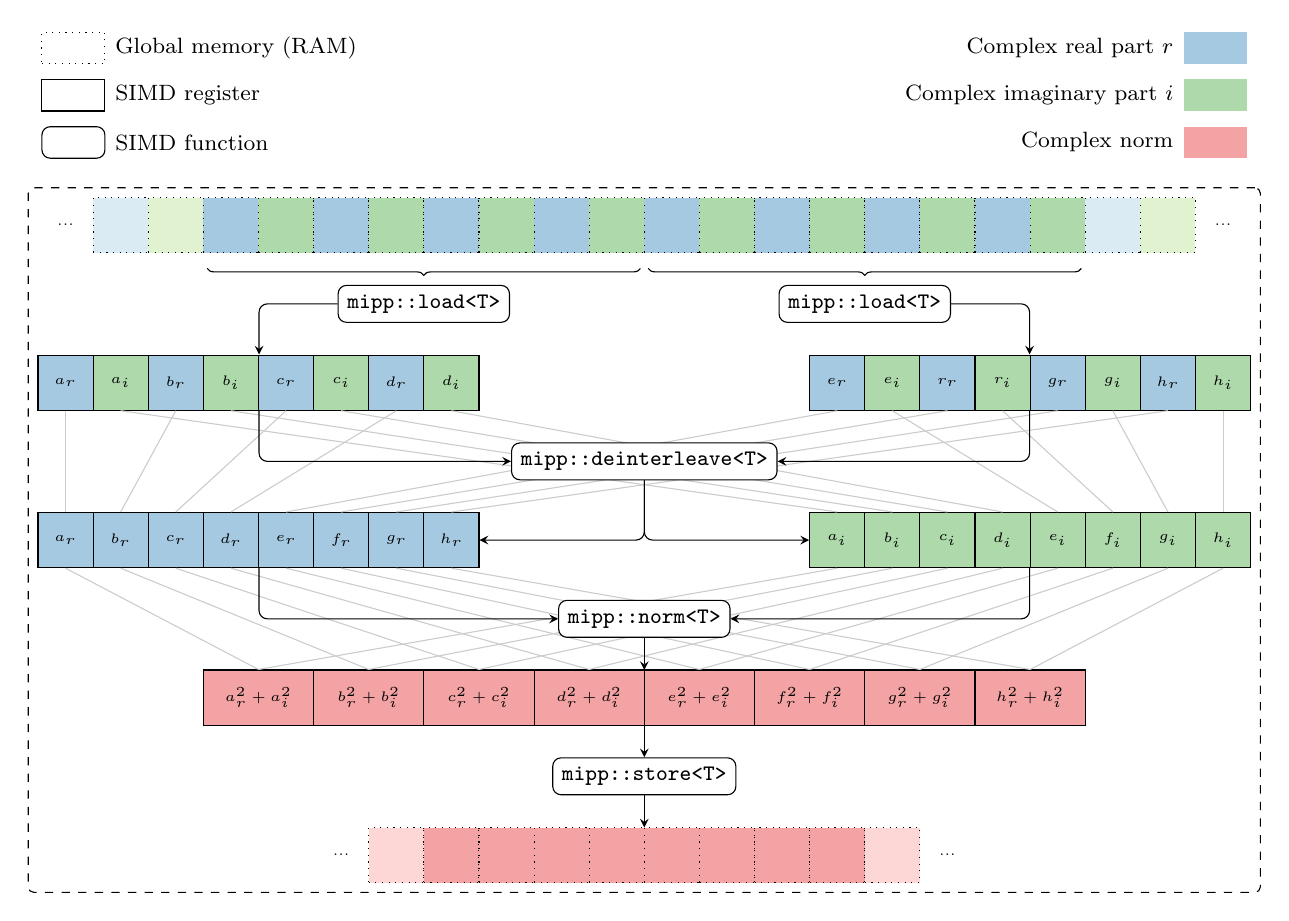
\begin{tikzpicture}[baseline]
    \tikzset{ er/.style ={draw=black, minimum width=0.7cm, minimum height=0.7cm, text=black, fill=Paired-1!40 } }
    \tikzset{ ei/.style ={draw=black, minimum width=0.7cm, minimum height=0.7cm, text=black, fill=Paired-3!40 } }
    \tikzset{ erd/.style={draw=black, minimum width=1.4cm, minimum height=0.7cm, text=black, fill=Paired-1!40 } }
    \tikzset{ eid/.style={draw=black, minimum width=1.4cm, minimum height=0.7cm, text=black, fill=Paired-3!40 } }
    \tikzset{ ers/.style={draw=black, minimum width=0.7cm, minimum height=0.7cm, text=black, fill=Paired-2!40 } }
    \tikzset{ eis/.style={draw=black, minimum width=0.7cm, minimum height=0.7cm, text=black, fill=Paired-4!40 } }
    \tikzset{ ex/.style ={draw=black, minimum width=0.7cm, minimum height=0.7cm, text=black, fill=Paired-6!40 } }
    \tikzset{ ey/.style ={draw=black, minimum width=0.7cm, minimum height=0.7cm, text=black, fill=Paired-5!40 } }
    \tikzset{ exd/.style={draw=black, minimum width=1.4cm, minimum height=0.7cm, text=black, fill=Paired-5!40 } }
    \tikzset{ ept/.style={            minimum width=0.7cm, minimum height=0.7cm]                              } }

    \tikzstyle{lnk}=[->,>=stealth,rounded corners=3pt]
    \tikzstyle{shf}=[black!20]
    \tikzstyle{intr}=[rounded corners=3pt, fill=white, draw=black]

    \newcommand\vs{2.0}
    \newcommand\lft{0.0}
    \newcommand\ctr{4.9}
    \newcommand\rth{9.8}

    \node[draw=black, dotted             , minimum width=0.8cm, minimum height=0.4cm, label={[black]right:\footnotesize{Global memory (RAM)}}] (ram)   at (0.1, -1.1+3.35) {};
    \node[draw=black,                    , minimum width=0.8cm, minimum height=0.4cm, label={[black]right:\footnotesize{SIMD register}}      ] (simdr) at (0.1, -1.7+3.35) {};
    \node[draw=black, rounded corners=3pt, minimum width=0.8cm, minimum height=0.4cm, label={[black]right:\footnotesize{SIMD function}}      ] (simdi) at (0.1, -2.3+3.35) {};

    \node[fill=Paired-1!40, minimum width=0.8cm, minimum height=0.4cm, label={[black]left:\footnotesize{Complex real part $r$}}     ] (cr) at (\rth+0.7+4.10, -1.1+3.35) {};
    \node[fill=Paired-3!40, minimum width=0.8cm, minimum height=0.4cm, label={[black]left:\footnotesize{Complex imaginary part $i$}}] (ci) at (\rth+0.7+4.10, -1.7+3.35) {};
    \node[fill=Paired-5!40, minimum width=0.8cm, minimum height=0.4cm, label={[black]left:\footnotesize{Complex norm}}              ] (cn) at (\rth+0.7+4.10, -2.3+3.35) {};

    \node[ept        ] (mi_er0)  at ( 0.0, 0.00) {\tiny{...}};
    \node[ers, dotted] (mi_er1)  at ( 0.7, 0.00) {};
    \node[eis, dotted] (mi_er2)  at ( 1.4, 0.00) {};
    \node[er , dotted] (mi_er3)  at ( 2.1, 0.00) {};
    \node[ei , dotted] (mi_er4)  at ( 2.8, 0.00) {};
    \node[er , dotted] (mi_er5)  at ( 3.5, 0.00) {};
    \node[ei , dotted] (mi_er6)  at ( 4.2, 0.00) {};
    \node[er , dotted] (mi_er7)  at ( 4.9, 0.00) {};
    \node[ei , dotted] (mi_er8)  at ( 5.6, 0.00) {};
    \node[er , dotted] (mi_er9)  at ( 6.3, 0.00) {};
    \node[ei , dotted] (mi_er10) at ( 7.0, 0.00) {};
    \node[er , dotted] (mi_er11) at ( 7.7, 0.00) {};
    \node[ei , dotted] (mi_er12) at ( 8.4, 0.00) {};
    \node[er , dotted] (mi_er13) at ( 9.1, 0.00) {};
    \node[ei , dotted] (mi_er14) at ( 9.8, 0.00) {};
    \node[er , dotted] (mi_er15) at (10.5, 0.00) {};
    \node[ei , dotted] (mi_er16) at (11.2, 0.00) {};
    \node[er , dotted] (mi_er17) at (11.9, 0.00) {};
    \node[ei , dotted] (mi_er18) at (12.6, 0.00) {};
    \node[ers, dotted] (mi_er19) at (13.3, 0.00) {};
    \node[eis, dotted] (mi_er20) at (14.0, 0.00) {};
    \node[ept        ] (mi_er21) at (14.7, 0.00) {\tiny{...}};

    \node[er] (r0_er0) at (\lft+0.0, -\vs) {\tiny{$a_r$}};
    \node[ei] (r0_er1) at (\lft+0.7, -\vs) {\tiny{$a_i$}};
    \node[er] (r0_er2) at (\lft+1.4, -\vs) {\tiny{$b_r$}};
    \node[ei] (r0_er3) at (\lft+2.1, -\vs) {\tiny{$b_i$}};
    \node[er] (r0_er4) at (\lft+2.8, -\vs) {\tiny{$c_r$}};
    \node[ei] (r0_er5) at (\lft+3.5, -\vs) {\tiny{$c_i$}};
    \node[er] (r0_er6) at (\lft+4.2, -\vs) {\tiny{$d_r$}};
    \node[ei] (r0_er7) at (\lft+4.9, -\vs) {\tiny{$d_i$}};

    \draw[decorate,decoration={brace,raise=0.2cm}] (\lft+ 7.0+0.30,-0.35) -- (\lft+2.1-0.30,-0.35);
    \draw[decorate,decoration={brace,raise=0.2cm}] (\lft+12.6+0.30,-0.35) -- (\lft+7.7-0.30,-0.35);

    \node[er] (r1_er0) at (\rth+0.0, -\vs) {\tiny{$e_r$}};
    \node[ei] (r1_er1) at (\rth+0.7, -\vs) {\tiny{$e_i$}};
    \node[er] (r1_er2) at (\rth+1.4, -\vs) {\tiny{$r_r$}};
    \node[ei] (r1_er3) at (\rth+2.1, -\vs) {\tiny{$r_i$}};
    \node[er] (r1_er4) at (\rth+2.8, -\vs) {\tiny{$g_r$}};
    \node[ei] (r1_er5) at (\rth+3.5, -\vs) {\tiny{$g_i$}};
    \node[er] (r1_er6) at (\rth+4.2, -\vs) {\tiny{$h_r$}};
    \node[ei] (r1_er7) at (\rth+4.9, -\vs) {\tiny{$h_i$}};

    \node[intr] (intr0) at (4.2+0.35, -\vs+1) {\footnotesize{\texttt{mipp::load<T>}}};
    \node[intr] (intr1) at (9.8+0.35, -\vs+1) {\footnotesize{\texttt{mipp::load<T>}}};

    \node[er] (r2_er0) at (\lft+0.0, -\vs-\vs) {\tiny{$a_r$}};
    \node[er] (r2_er1) at (\lft+0.7, -\vs-\vs) {\tiny{$b_r$}};
    \node[er] (r2_er2) at (\lft+1.4, -\vs-\vs) {\tiny{$c_r$}};
    \node[er] (r2_er3) at (\lft+2.1, -\vs-\vs) {\tiny{$d_r$}};
    \node[er] (r2_er4) at (\lft+2.8, -\vs-\vs) {\tiny{$e_r$}};
    \node[er] (r2_er5) at (\lft+3.5, -\vs-\vs) {\tiny{$f_r$}};
    \node[er] (r2_er6) at (\lft+4.2, -\vs-\vs) {\tiny{$g_r$}};
    \node[er] (r2_er7) at (\lft+4.9, -\vs-\vs) {\tiny{$h_r$}};

    \node[ei] (r3_er0) at (\rth+0.0, -\vs-\vs) {\tiny{$a_i$}};
    \node[ei] (r3_er1) at (\rth+0.7, -\vs-\vs) {\tiny{$b_i$}};
    \node[ei] (r3_er2) at (\rth+1.4, -\vs-\vs) {\tiny{$c_i$}};
    \node[ei] (r3_er3) at (\rth+2.1, -\vs-\vs) {\tiny{$d_i$}};
    \node[ei] (r3_er4) at (\rth+2.8, -\vs-\vs) {\tiny{$e_i$}};
    \node[ei] (r3_er5) at (\rth+3.5, -\vs-\vs) {\tiny{$f_i$}};
    \node[ei] (r3_er6) at (\rth+4.2, -\vs-\vs) {\tiny{$g_i$}};
    \node[ei] (r3_er7) at (\rth+4.9, -\vs-\vs) {\tiny{$h_i$}};

    \draw[shf] (r0_er0.south) -- (r2_er0.north);
    \draw[shf] (r0_er1.south) -- (r3_er0.north);
    \draw[shf] (r0_er2.south) -- (r2_er1.north);
    \draw[shf] (r0_er3.south) -- (r3_er1.north);
    \draw[shf] (r0_er4.south) -- (r2_er2.north);
    \draw[shf] (r0_er5.south) -- (r3_er2.north);
    \draw[shf] (r0_er6.south) -- (r2_er3.north);
    \draw[shf] (r0_er7.south) -- (r3_er3.north);

    \draw[shf] (r1_er0.south) -- (r2_er4.north);
    \draw[shf] (r1_er1.south) -- (r3_er4.north);
    \draw[shf] (r1_er2.south) -- (r2_er5.north);
    \draw[shf] (r1_er3.south) -- (r3_er5.north);
    \draw[shf] (r1_er4.south) -- (r2_er6.north);
    \draw[shf] (r1_er5.south) -- (r3_er6.north);
    \draw[shf] (r1_er6.south) -- (r2_er7.north);
    \draw[shf] (r1_er7.south) -- (r3_er7.north);

    \draw[lnk] (intr0.west) -| (r0_er3.north east);
    \draw[lnk] (intr1.east) -| (r1_er4.north west);

    \node[intr] (intr2) at (7.35, -\vs-\vs+1) {\footnotesize{\texttt{mipp::deinterleave<T>}}};


    \draw[lnk] (r0_er3.south east) |- (intr2.west);
    \draw[lnk] (r1_er4.south west) |- (intr2.east);

    \draw[lnk] (intr2) |- (r2_er7.east);
    \draw[lnk] (intr2) |- (r3_er0.west);

    \newcommand\ctrd{2.45}

    \node[exd] (r6_er0) at (\ctrd+0.0, -\vs-\vs-\vs) {\tiny{$a_r^2+a_i^2$}};
    \node[exd] (r6_er1) at (\ctrd+1.4, -\vs-\vs-\vs) {\tiny{$b_r^2+b_i^2$}};
    \node[exd] (r6_er2) at (\ctrd+2.8, -\vs-\vs-\vs) {\tiny{$c_r^2+c_i^2$}};
    \node[exd] (r6_er3) at (\ctrd+4.2, -\vs-\vs-\vs) {\tiny{$d_r^2+d_i^2$}};
    \node[exd] (r6_er4) at (\ctrd+5.6, -\vs-\vs-\vs) {\tiny{$e_r^2+e_i^2$}};
    \node[exd] (r6_er5) at (\ctrd+7.0, -\vs-\vs-\vs) {\tiny{$f_r^2+f_i^2$}};
    \node[exd] (r6_er6) at (\ctrd+8.4, -\vs-\vs-\vs) {\tiny{$g_r^2+g_i^2$}};
    \node[exd] (r6_er7) at (\ctrd+9.8, -\vs-\vs-\vs) {\tiny{$h_r^2+h_i^2$}};

    \draw[shf] (r2_er0.south) -- (r6_er0.north);
    \draw[shf] (r2_er1.south) -- (r6_er1.north);
    \draw[shf] (r2_er2.south) -- (r6_er2.north);
    \draw[shf] (r2_er3.south) -- (r6_er3.north);
    \draw[shf] (r2_er4.south) -- (r6_er4.north);
    \draw[shf] (r2_er5.south) -- (r6_er5.north);
    \draw[shf] (r2_er6.south) -- (r6_er6.north);
    \draw[shf] (r2_er7.south) -- (r6_er7.north);
    \draw[shf] (r3_er0.south) -- (r6_er0.north);
    \draw[shf] (r3_er1.south) -- (r6_er1.north);
    \draw[shf] (r3_er2.south) -- (r6_er2.north);
    \draw[shf] (r3_er3.south) -- (r6_er3.north);
    \draw[shf] (r3_er4.south) -- (r6_er4.north);
    \draw[shf] (r3_er5.south) -- (r6_er5.north);
    \draw[shf] (r3_er6.south) -- (r6_er6.north);
    \draw[shf] (r3_er7.south) -- (r6_er7.north);

    \node[intr] (intr3) at (7.35, -\vs-\vs-\vs+1) {\footnotesize{\texttt{mipp::norm<T>}}};

    \draw[lnk] (r2_er3.south east) |- (intr3.west);
    \draw[lnk] (r3_er4.south west) |- (intr3.east);

    \draw[lnk] (intr3) -- (7.35,-\vs-\vs-\vs+0.35);

    \node[ept        ] (mo_er5)  at ( 3.5, -\vs-\vs-\vs-\vs) {\tiny{...}};
    \node[ex , dotted] (mo_er6)  at ( 4.2, -\vs-\vs-\vs-\vs) {};
    \node[ey , dotted] (mo_er7)  at ( 4.9, -\vs-\vs-\vs-\vs) {};
    \node[ey , dotted] (mo_er8)  at ( 5.6, -\vs-\vs-\vs-\vs) {};
    \node[ey , dotted] (mo_er9)  at ( 6.3, -\vs-\vs-\vs-\vs) {};
    \node[ey , dotted] (mo_er10) at ( 7.0, -\vs-\vs-\vs-\vs) {};
    \node[ey , dotted] (mo_er11) at ( 7.7, -\vs-\vs-\vs-\vs) {};
    \node[ey , dotted] (mo_er12) at ( 8.4, -\vs-\vs-\vs-\vs) {};
    \node[ey , dotted] (mo_er13) at ( 9.1, -\vs-\vs-\vs-\vs) {};
    \node[ey , dotted] (mo_er14) at ( 9.8, -\vs-\vs-\vs-\vs) {};
    \node[ex , dotted] (mo_er15) at (10.5, -\vs-\vs-\vs-\vs) {};
    \node[ept        ] (mo_er16) at (11.2, -\vs-\vs-\vs-\vs) {\tiny{...}};

    \node[intr] (intr4) at (7.35, -\vs-\vs-\vs-\vs+1) {\footnotesize{\texttt{mipp::store<T>}}};

    \draw[lnk] (7.35,-\vs-\vs-\vs-0.35) -- (intr4);
    \draw[lnk] (intr4) -- (7.35,-\vs-\vs-\vs-\vs+0.35);

    \node[draw=black, rounded corners=2pt, dashed, fit=(mo_er14) (mi_er0) (r2_er0) (r3_er7)] {};
  \end{tikzpicture}
\end{document}